\documentclass[12pt]{report}
\usepackage[utf8]{inputenc}
%\usepackage[14pt]{extsizes}
\usepackage{listings}
\usepackage{indentfirst}
\usepackage{geometry}
\usepackage{textcomp}
\usepackage{amssymb}
\usepackage{amsmath}
\usepackage{amsthm} 
\usepackage{caption}
\usepackage{misccorr}
\usepackage[noadjust]{cite}
\usepackage{cmap} 
\usepackage[T2A]{fontenc}
\usepackage[english, russian]{babel}
\usepackage{graphics}
\usepackage{graphicx}
\usepackage{textcomp}
\usepackage{verbatim}
\usepackage{makeidx}
\usepackage{float}
\usepackage{bm}
\usepackage{esint}
\usepackage{mathtools}
\usepackage{graphicx}
\usepackage{listings}
% Для листинга кода:
\lstset{ %
language=python,                 % выбор языка для подсветки (здесь это С)
basicstyle=\small\sffamily, % размер и начертание шрифта для подсветки кода
numbers=left,               % где поставить нумерацию строк (слева\справа)
numberstyle=\tiny,           % размер шрифта для номеров строк
stepnumber=1,                   % размер шага между двумя номерами строк
numbersep=5pt,                % как далеко отстоят номера строк от подсвечиваемого кода
showspaces=false,            % показывать или нет пробелы специальными отступами
showstringspaces=false,      % показывать или нет пробелы в строках
showtabs=false,             % показывать или нет табуляцию в строках
frame=single,              % рисовать рамку вокруг кода
tabsize=2,                 % размер табуляции по умолчанию равен 2 пробелам
captionpos=t,              % позиция заголовка вверху [t] или внизу [b] 
breaklines=true,           % автоматически переносить строки (да\нет)
breakatwhitespace=false, % переносить строки только если есть пробел
escapeinside={\#*}{*)}   % если нужно добавить комментарии в коде
}


% plot
\usepackage{pgfplots}
\usepackage{filecontents}
\usetikzlibrary{datavisualization}
\usetikzlibrary{datavisualization.formats.functions}

% Для измененных титулов глав:
\usepackage{titlesec, blindtext, color} % подключаем нужные пакеты
\definecolor{gray75}{gray}{0.75} % определяем цвет
\newcommand{\hsp}{\hspace{20pt}} % длина линии в 20pt
% titleformat определяет стиль
\titleformat{\chapter}[hang]{\Huge\bfseries}{\thechapter\hsp\textcolor{gray75}{|}\hsp}{0pt}{\Huge\bfseries}

\makeatletter
\def\@biblabel#1{#1. }
\makeatother

\usepackage{hyperref}

\newcommand{\specchapter}[1]{\chapter*{#1}\addcontentsline{toc}{chapter}{#1}}
\newcommand{\specsection}[1]{\section*{#1}\addcontentsline{toc}{section}{#1}}
\newcommand{\specsubsection}[1]{\subsection*{#1}\addcontentsline{toc}{subsection}{#1}}

% геометрия
\geometry{pdftex, left = 2cm, right = 2cm, top = 2.5cm, bottom = 2.5cm}

\titlespacing{\chapter}{0pt}{-30pt}{20pt}

\setcounter{tocdepth}{4} % фикс переноса 
\righthyphenmin = 2
\tolerance = 2048

\begin{document}
%\def\chaptername{} % убирает "Глава"
\thispagestyle{empty}
\renewcommand\bibname{Список литературы}

\vspace{\baselineskip}
\noindent \begin{minipage}{0.15\textwidth}
	
\includegraphics[width=\linewidth]{bmstu}
\end{minipage}
\noindent\begin{minipage}{0.9\textwidth}
	\centering
	\textbf{Министерство науки и высшего образования Российской Федерации}\\
	\textbf{Федеральное государственное бюджетное образовательное учреждение высшего образования}\\
	\textbf{«Московский государственный технический университет имени Н.Э.~Баумана}\\
	\textbf{(национальный исследовательский университет)»}\\
	\textbf{(МГТУ им. Н.Э.~Баумана)}
\end{minipage}

\noindent\rule{18cm}{3pt}
\newline\newline
\noindent ФАКУЛЬТЕТ $\underline{\text{«Информатика и системы управления»}}$ \newline\newline
\noindent КАФЕДРА $\underline{\text{«Программное обеспечение ЭВМ и информационные технологии»}}$\newline\newline\newline\newline\newline\newline\newline


\begin{center}
\Large\textbf{Лабораторная работа № 3}
\end{center}
\vspace{\baselineskip}
\noindent\textbf{Дисциплина} $\underline{\text{Анализ алгоритмов~~~~~~~~~~~~~~~~~~~~~~~~~~~~~~~}}$\newline\newline
\noindent\textbf{Тема} $\underline{\text{Трудоемкость алгоритмов сортировки~~~~~~~~~~~~~~~~~}}$\newline\newline
\noindent\textbf{Студент} $\underline{\text{Куликов Д. А.~~~~~~~~~~~~~~~~~~~~~~~~~~~~~~~~~~~~~~~~~~~~~}}$\newline\newline
\noindent\textbf{Группа} $\underline{\text{ИУ7-52Б~~~~~~~~~~~~~~~~~~~~~~~~~~~~~~~~~~~~~~~~~~~~~~~~~~~~~~}}$\newline\newline
\noindent\textbf{Оценка (баллы)} $\underline{\text{~~~~~~~~~~~~~~~~~~~~~~~~~~~~~~~~~~~~~~~~~~~~~~~~~~~~~}}$\newline\newline
\noindent\textbf{Преподаватель} $\underline{\text{Волкова Л. Л.~~~~~~~~~~~~~~~~~~~~~~~~~~~~~~~~~~~}}$\newline

\begin{center}
	\vfill
	Москва~---~\the\year
	~г.
\end{center}
\clearpage

\tableofcontents

\newpage
\chapter*{Введение}
\addcontentsline{toc}{chapter}{Введение}
Алгоритмы сортировки имеют большое практическое применение.
Их можно встретить почти везде, где речь идет об обработке и хранении больших объемов информации.
Сортировки используются в самом широком спектре задач, включая обработку коммерческих, сейсмических, космических и прочих данных \cite{academy}.
Часто сортировка является просто вспомогательной операцией для упорядочивания данных, упрощения последующих алгебраических действий над данными и т. п.

Сортировка применяется во всех без исключения областях программирования, например, базы данных или математические программы.
Упорядоченные объекты содержатся в телефонных книгах, ведомостях налогов, в библиотеках, в оглавлениях, в словарях.

В настоящее время, в связи с экспоненциально возросшими объемами данных, вопрос эффективной сортировки данных снова стал актуальным.\vspace{\baselineskip} 


\textbf{Цель работы:} оценить трудоемкость алгоритмов сортировки массива и получить практический навык реализации алгоритмов.\vspace{\baselineskip} 

\textbf{Задачи работы:}
\begin{enumerate}
  	\item изучить алгоритмы сортировки массива: пузырьком, вставка и выбором; 
  	\item оценить трудоемкость данных алгоритмов сортировки;
  	\item реализовать данные алгоритмы сортировки массива на одном из языков программирования;  
  	\item сравнить алгоритмы сортировки массива.
\end{enumerate}


\chapter{Аналитическая часть}

Сортировка массива — одна из самых частых операций над массивом. Алгоритмы реализуют упорядочивание элементов в списке. В случае, когда элемент списка имеет несколько полей, поле, служащее критерием порядка, называется ключом сортировки. На практике в качестве ключа
часто выступает число, а в остальных полях хранятся какие-либо данные,
никак не влияющие на работу алгоритма.


\section{Описание алгоритма сортировки «пузырьком»}
Алгоритм состоит из повторяющихся проходов по сортируемому массиву.
За каждый проход элементы последовательно сравниваются попарно, и если
порядок в паре неверный, выполняется обмен элементов. Проходы по массиву
повторяются раз или до тех пор, пока на очередном проходе не окажется,
что обмены больше не нужны, что означает массив отсортирован. При каждом
проходе алгоритма по внутреннему циклу, очередной наибольший элемент
массива ставится на своё место в конце массива рядом с предыдущим
«наибольшим элементом», а наименьший элемент перемещается на одну
позицию к началу массива («всплывает» до нужной позиции, как пузырёк в
воде — отсюда и название алгоритма). 

\section{Описание алгоритма сортировки вставками}

Сортировка вставками — алгоритм сортировки, котором элементы входной последовательности просматриваются по одному, и каждый новый поступивший элемент размещается в подходящее место среди ранее упорядоченных элементов \cite{habr}.

В начальный момент отсортированная последовательность пуста.
На каждом шаге алгоритма выбирается один из элементов входных данных и помещается на нужную позицию в уже отсортированной последовательности до тех пор, пока набор входных данных не будет исчерпан.
В любой момент времени в отсортированной последовательности элементы удовлетворяют требованиям к выходным данным алгоритма.

На рис. 1.1 показаны этапы сортировки вставками массива [18, 20,
5, 13, 15].

\newpage
\begin{figure}[h]
	\center{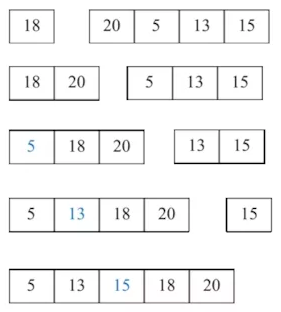
\includegraphics[scale=0.7]{insSortExample}}
	\caption{Сортировка вставками}
	\label{figure:image}
\end{figure}

\section{Описание алгоритма сортировки выбором}

Сначала нужно рассмотреть подмножество массива и найти в нём
максимум (или минимум). Затем выбранное значение меняют местами со
значением первого неотсортированного элемента. Таким образом, после i-ой итерации первые i элементов будут стоять на своих местах. Этот шаг
нужно повторять до тех пор, пока в массиве не закончатся неотсортированные подмассивы.
Нужно отметить, что эту сортировку можно реализовать двумя способами – сохраняя минимум и его индекс или просто переставляя текущий
элемент с рассматриваемым, если они стоят в неправильном порядке. 

На рис. 1.2 показаны этапы сортировки выбором массива [4, 9, 7,
6, 2, 3].
\newpage
\begin{figure}[h]
	\center{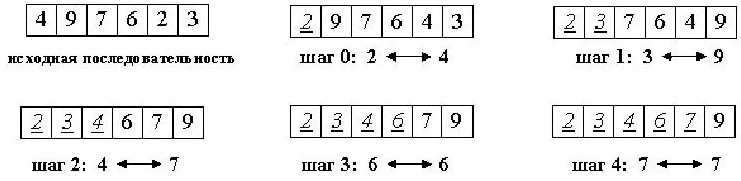
\includegraphics[scale=0.7]{selSortExample}}
	\caption{Сортировка выбором}
	\label{figure:image}
\end{figure}

\chapter{Конструкторская часть}
В этом разделе содержатся cхемы алгоритмов сортировки массива.
На вход алгоритмы принимают массив и размер массива. На выходе выдают отсортированный массив.\vspace{\baselineskip}
	
\section{Схемы алгоритмов}
На рис. 2.1-2.3 приведены схемы следующих алгоритмов:
\begin{enumerate}
	\item алгоритм сортировки массива «пузырьком»;
	\item алгоритм сортировки массива вставками;
	\item алгоритм сортировки массива выбором.
\end{enumerate}

\newpage
\begin{figure}[h]
	\center{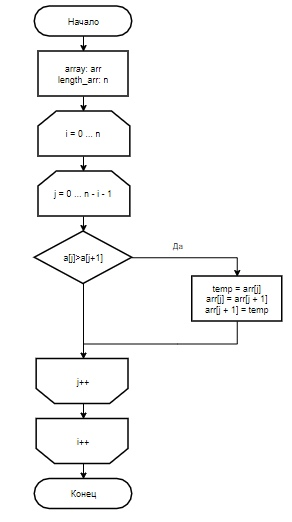
\includegraphics[scale=1]{schemeBubbleSort}}
	\caption{Алгоритм сортировки массива «пузырьком»}
	\label{figure:image}
\end{figure}

\newpage
\begin{figure}[h]
	\center{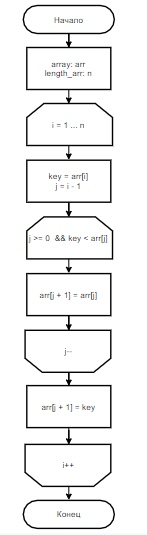
\includegraphics[scale=1]{schemeInsertSort}}
	\caption{Алгоритм сортировки массива вставками}
	\label{figure:image}
\end{figure}

\newpage
\begin{figure}[h]
	\center{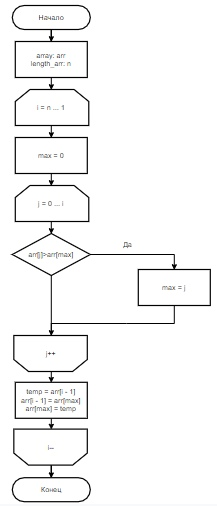
\includegraphics[scale=1]{schemeSelSort}}
	\caption{Алгоритм сортировки массива выбором}
	\label{figure:image}
\end{figure}



\chapter{Технологическая часть}
В данном разделе будут рассмотрены требования к программному обеспечению, средства реализации, представлен листинг кода, трудоемкость алгоритмов и описание тестирования.
\section{Требования к программному обеспечению}
\textbf{Требования к вводу:} на вход подаются массив и размер массива.\vspace{\baselineskip} 

\textbf{Требования к программе:}
\begin{enumerate}
	\item на выходе
	необходимо получить отсортированный массив;
	\item требуется замерить время работы
	каждого из алгоритмов. 
\end{enumerate}
\section{Средства реализации}
В качестве языка программирования был выбран Python т.к. я знаком с данным языком, он простой и лаконичный, имеющий немногословный и понятный синтаксис, похожий на псевдокод, обладающий сильной динамической типизацией, которая способствует быстрому написанию кода. 

Среда разработки — PyCharm, которая предоставляет умную проверку кода, быстрое выявление ошибок и оперативное исправление, вкупе с автоматическим рефакторингом кода, и богатыми возможностями в навигации.  

Время  работы алгоритмов было замерено с помощью функции process\_time() из библиотеки time \cite{time}.

\newpage
\section{Листинг кода}

В листингах 3.1-3.3 представлена реализация алгоритмов сортировки массива.
\vspace{\baselineskip}

\begin{lstlisting}[label=some-code,caption=Сортировка массива «пузырьком»]
def BubbleSort(a, n):
	i = 0
	while i < n:
		j = 0
		while j < n - i - 1:
			if a[j] > a[j + 1]:
				temp = a[j]
				a[j] = a[j + 1]
				a[j + 1] = temp
			j += 1
		i += 1
\end{lstlisting}

\begin{lstlisting}[label=some-code,caption=Сортировка массива вставками]
def InsertSort(a, n):
	i = 1
	while i < n:
		key = a[i]
		j = i - 1
		while j >= 0 and key < a[j]:
			a[j + 1] = a[j]
			j -= 1
		a[j + 1] = key
		i += 1
\end{lstlisting}

\newpage
\begin{lstlisting}[label=some-code,caption=Сортировка массива выбором]
def SelectionSort(a, n):
	i = n
	while i > 1:
		maximum = 0
		j = 0
		while j < i:
			if a[j] > a[maximum]:
				maximum = j
			j += 1
		temp = a[i - 1]
		a[i - 1] = a[maximum]
		a[maximum] = temp
		i -= 1
\end{lstlisting}

\newpage
\section{Трудоемкость алгоритмов}
Введем модель вычисления трудоемкости для оценки алгоритмов: 
\begin{itemize}
	\item базовые операции стоимостью 1 — +, -, *, /, =, ==, <=, >=, !=, +=, [], получение полей класса
	\item оценка трудоемкости цикла: Fц = init +  N*(a + Fтела + post) + a, где a - условие цикла, init - предусловие цикла, post - постусловие цикла
	\item стоимость условного перехода применим за 0, стоимость вычисления условия остаётся
\end{itemize}

Оценим трудоемкость алгоритмов сортировки массива по коду программы.

\subsection{Трудоемкость алгоритма сортировки «пузырьком»}
Рассмотрим трудоемкость алгоритма сортировки «пузырьком».\vspace{\baselineskip} 

Наилучший случай: 2 + (N - 1) * (3 + 1 + 2 + (N / 2) * 8) = 4 * N * N + 2 * N - 6

Наихудший случай: 2 + (N - 1) * (3 + 1 + 2 + (N / 2) * (8 + 9)) = 8,5 * N * N - 2,5 * N - 4

\subsection{Трудоемкость алгоритма сортировки вставками}
Рассмотрим трудоемкость алгоритма сортировки вставками.\vspace{\baselineskip} 

Наилучший случай: 2 + N * (2 + 2 + 3 + 6) = 13 * N + 2 \vspace{\baselineskip}

Наихудший случай: 2 + N * (2 + 2 + 3 + 6 + (N - 1) / 4 * (5 + 4)) = 4.5 * N * N + 8.5 * * N + 2

\subsection{Трудоемкость алгоритма сортировки выбором}
Рассмотрим трудоемкость алгоритма сортировки выбором.\vspace{\baselineskip} 

Наилучший случай: 2 + (N - 1) * (3 + 11 + 2 + (N / 2) * (2 + 3)) = 2,5 * N * N + 12,5 * *N - 13  

Наихудший случай: 2 + (N - 1) * (3 + 11 + 2 + (N / 2) * (2 + 3 + 1)) = 3 * N * N + 12 * *N - 13

\newpage
\section{Тестирование}
Реализовано функциональное тестирование отдельным файлом test.py. Полученные результаты функций сравниваются с контрольными значениями. \vspace{\baselineskip}

В таблице 3.1 представлены функциональные тесты для проверки работы программы.

\begin{table}[H]
	\caption{\label{tabular:functional_test} Функциональные тесты}
	\begin{center}
		
			\begin{tabular}{ | l | l | }
			\hline
			Входные данные & Ожидаемый результат\\
			\hline
			0 0 0 0 0 & 0 0 0 0 0\\
			1 2 3 4 5 & 1 2 3 4 5 \\
			5 4 3 2 1 & 1 2 3 4 5 \\
			4 2 3 5 1 & 1 2 3 4 5 \\
			3 2 3 2 3 2 & 2 2 2 3 3 3 \\
			\hline
		\end{tabular}
	\end{center}
\end{table} 

Программа успешно прошла все тестовые случаи.

\chapter{Экспериментальная часть}

В данном разделе приведены примеры работы программы и сравнительный анализ алгоритмов на основе экспериментальных данных. 

\section{Примеры работы} 
 
На рис. 4.1 представлено пример работы программы. 

\begin{figure}[h]
	\center{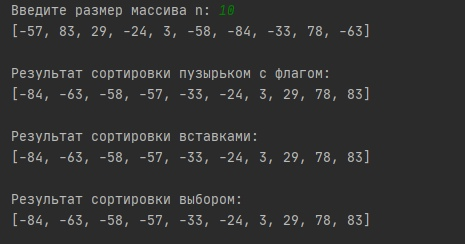
\includegraphics[scale=0.7]{demonstrate}}
	\caption{Результат сортировки массива длиной 10}
	\label{figure:image}
\end{figure}

\newpage
\section{Постановка эксперимента по замеру времени}

Для произведения замеров времени выполнения реализации алгоритмов будет использована формула: \begin{equation}\label{eq:fourierrow}
	t = \frac{T}{N}
\end{equation}
где t — среднее время выполнения алгоритма, N — количество замеров, T — время выполнения N замеров.  
Неоднократное измерение времени необходимо для получения более точного результа.  
 
 Количество замеров взято равным 100. Эксперимент проводится на квадратных матрицах, заполненных произвольными значениями.
 
 Был проведен замер времени работы каждого из алгоритмов, результат представлен в Таблицах 4.1 - 4.2. \vspace{\baselineskip}
 
В таблице 4.1 представлены замеры времени работы алгоритмов в произвольном случае.

\begin{table}[H]
	\caption{\label{tabular:rand} Время работы алгоритмов в произвольном случае}
	\begin{center}
		
		\begin{tabular}{ | l | l | l | l | l | }
			\hline
			длина & пузырьком, сек & выбором, сек & вставками, сек\\
			\hline
			100 & 0.00217266 & 0.00111016 & 0.00097969 \\
			250 & 0.01693750 & 0.00814063 & 0.00745312 \\
			500 & 0.05468750 & 0.02512700 & 0.02437500 \\
			1000 & 0.08968350 &  0.06523400  & 0.06078570 \\
			\hline
		\end{tabular}
	\end{center}
\end{table} 

 В таблице 4.2 представлены замеры времени работы алгоритмов в наилучшем и нахудшим случаях на примере массива размера 100

\begin{table}[H]
	\caption{\label{tabular:rand} Время работы алгоритмов в наилучшем и нахудшим случаях}
	\begin{center}
		
		\begin{tabular}{ | l | l | l | }
			\hline
			сортировка & размер массива & время, сек\\
			\hline
			пузырьком(наилучший случай) & 100 & 0.00140312 \\
			пузырьком(наихудший случай) & 100 & 0.00251406 \\
			выбором(наилучший случай) & 100 & 0.00105469 \\
			выбором(наихудший случай) & 100 & 0.00146719 \\
			вставками(наилучший случай) & 100 & 0.00003906 \\
			вставками(наихудший случай) & 100 & 0.00262031\\
			\hline
		\end{tabular}
	\end{center}
\end{table} 

\newpage
\textbf{Вывод: } 
При работе с упорядоченными или практически упорядоченными следует использовать сортировку вставкой (при выборе из трех предложенных алгоритмов). Сортировка выбором показывает стабильный результат, практически независимый от входных данных, в отличии от сортировки вставкой, время которой сильно разбросано. Время сортировки пузырьком имеет меньший разброс, однако из-за того, что верхний предел совпадает с пределом сортировки вставкой, мы можем сказать, что сортировка вставкой в среднем будет лучше сортировки пузырьком. С учетом посчитанных трудоемкостей алгоритмов сортировки, для массива больших размеров следует использовать алгоритм сортировки вставками

\chapter*{Заключение}
\addcontentsline{toc}{chapter}{Заключение}

В ходе работы были изучены алгоритмы сортировки массива. Реализованы 3 алгоритма: пузырьком, вставка, выбор. Приведен программный код реализации этих алгоритмов.

Была подсчитана трудоемкость каждого из алгоритмов. А также было проведено сравнение их по времени и трудоемкости.

Цель работы достигнута. Получены практические навыки реализации алгоритмов сортировки, а также проведена исследовательская работа по вычислению трудоемкости алгоритмов.


\begin{thebibliography}{2}
	\addcontentsline{toc}{chapter}{Список литературы}
	\bibitem{academy} Основные виды сортировок и примеры их реализации. [электронный ресурс]. Режим доступа: https://academy.yandex.ru/posts/osnovnye-vidy-sortirovok-i-primery-ikh-realizatsii
	(Дата обращения: 16.10.2020)
	
	\bibitem{habr} Описание алгоритмов сортировки и сравнение их производительности. [электронный ресурс] Режим доступа:
	https://habr.com/ru/post/335920/
	(Дата обращения: 16.10.2020)
	
	\bibitem{time} Официальный сайт Python, документация [электронный ресурс]. Режим доступа: https://docs.python.org/3/library/time.html, свободный (Дата обращения: 16.09.20)
	
\end{thebibliography}
\end{document}